\documentclass[12pt,a4paper,titlepage]{article}
\usepackage[utf8]{inputenc}
\usepackage[french]{babel}
\usepackage[T1]{fontenc}
\usepackage{amsmath}
\usepackage{amsfonts}
\usepackage{amssymb}
\usepackage{graphicx}
\usepackage{url}
\author{TRAN Quoc Nhat Han - Andrien Wartelle}
\title{Test paramétrique et de l'estimation de la loi géométrique et de Cauchy}
\usepackage{color}
\usepackage{listings}
\lstset{
language=R,
basicstyle=\scriptsize\ttfamily,
commentstyle=\ttfamily\color{green},
numbers=left,
numberstyle=\ttfamily\color{black}\footnotesize,
stepnumber=1,
numbersep=5pt,
backgroundcolor=\color{white},
showspaces=false,
showstringspaces=false,
showtabs=false,
frame=single,
tabsize=2,
captionpos=b,
breaklines=true,
breakatwhitespace=false,
keywordstyle=\color{blue},
stringstyle=\color{magenta},
literate=
  {á}{{\'a}}1 {é}{{\'e}}1 {í}{{\'i}}1 {ó}{{\'o}}1 {ú}{{\'u}}1
  {Á}{{\'A}}1 {É}{{\'E}}1 {Í}{{\'I}}1 {Ó}{{\'O}}1 {Ú}{{\'U}}1
  {à}{{\`a}}1 {è}{{\`e}}1 {ì}{{\`i}}1 {ò}{{\`o}}1 {ù}{{\`u}}1
  {À}{{\`A}}1 {È}{{\'E}}1 {Ì}{{\`I}}1 {Ò}{{\`O}}1 {Ù}{{\`U}}1
  {ä}{{\"a}}1 {ë}{{\"e}}1 {ï}{{\"i}}1 {ö}{{\"o}}1 {ü}{{\"u}}1
  {Ä}{{\"A}}1 {Ë}{{\"E}}1 {Ï}{{\"I}}1 {Ö}{{\"O}}1 {Ü}{{\"U}}1
  {â}{{\^a}}1 {ê}{{\^e}}1 {î}{{\^i}}1 {ô}{{\^o}}1 {û}{{\^u}}1
  {Â}{{\^A}}1 {Ê}{{\^E}}1 {Î}{{\^I}}1 {Ô}{{\^O}}1 {Û}{{\^U}}1
  {œ}{{\oe}}1 {Œ}{{\OE}}1 {æ}{{\ae}}1 {Æ}{{\AE}}1 {ß}{{\ss}}1
  {ű}{{\H{u}}}1 {Ű}{{\H{U}}}1 {ő}{{\H{o}}}1 {Ő}{{\H{O}}}1
  {ç}{{\c c}}1 {Ç}{{\c C}}1 {ø}{{\o}}1 {å}{{\r a}}1 {Å}{{\r A}}1
  {€}{{\EUR}}1 {£}{{\pounds}}1
}
\numberwithin{equation}{section}
\begin{document}
\maketitle 
\renewcommand{\contentsname}{Sommaire}
\tableofcontents

\clearpage

\begin{abstract}
Ce rapport est à montrer l'application de certaines tests statistiques pour la loi géométrique et la loi de Cauchy. Chaque section consiste de trois étapes séparées:
\begin{enumerate}
\item \emph{Estimer les paramètres inconnus}
\item \emph{Test de l'estimation}
\item \emph{Test d'adéquation}
\end{enumerate}
\end{abstract}

\section{Loi de Cauchy}
\subsection{Rappel}
Soit $f_X$ la fonction de densité de Cauchy de deux paramètres $x_0$ et $a$ ($a>0$), définie par:
\begin{equation}
\label{dCauchy}
{f_X}\left( x \right) = \frac{1}{{\pi a\left( {1 + {{\left( {\frac{{x - {x_0}}}{a}} \right)}^2}} \right)}} = \frac{1}{\pi }\frac{a}{{{{\left( {x - {x_0}} \right)}^2} + a}}
\end{equation}

\begin{figure}[h]
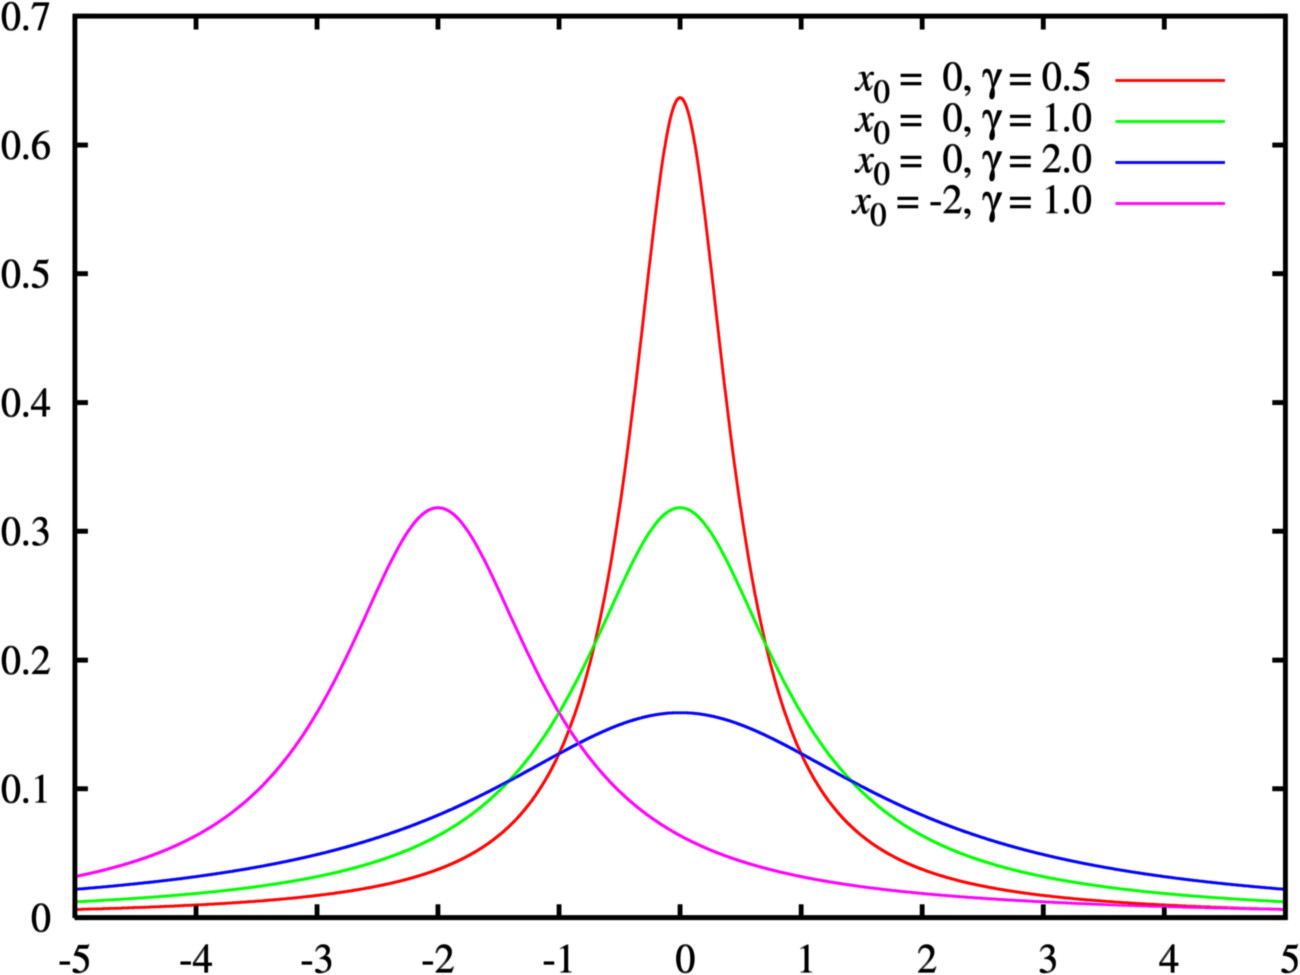
\includegraphics[width=\linewidth]{images/Cauchy_distribution_theoretic.png}
\caption{Distribution théorique de la loi Cauchy. Source : \cite{WikiLoiCauchy}}
\end{figure}

$a$ est dite l'échelle de la fonction, et $x_0$ est son médian.

La loi de Cauchy n'admet ni espérance ni écart type.

La fonction de répartition:
\begin{equation}
\label{rCauchy}
{F_X}\left( x \right) = \frac{1}{\pi }\arctan \left( {\frac{{x - {x_0}}}{a}} \right) + \frac{1}{2}
\end{equation}

\subsection{Estimer les paramètres inconnus}

\subsubsection*{Calcul théorique}

Soient $n$ réalisations $x_1, x_2, ..., x_n$. Assumons que ces données suivent la loi de Cauchy \eqref{dCauchy}.

Nous allons utiliser la méthode de maximum de rapport de vraisemblance.

En l'absence d'information de la distribution, nous assumons que ces mesures sont indépendants. Posons une variable aléatoire $X_i$ correspondante à chaque réalisation $x_i$ pour $i=\overline{1, n}$.

On écrit la loi conjointe de ces $n$ variables:

\begin{align*}
L (X) = L\left( {{X_1},{X_2},...,{X_n}} \right) & = \prod\limits_{i = 1}^n {{f_X}\left( {{X_i}} \right)} \\
& = \prod\limits_{i = 1}^n {\frac{1}{\pi }\frac{a}{{{{\left( {{x_i} - {x_0}} \right)}^2} + a}}} \\
& = {\pi ^{ - n}}\prod\limits_{i = 1}^n {\frac{a}{{{{\left( {{x_i} - {x_0}} \right)}^2} + a}}}
\end{align*}

On cherche l'optimum maximale.

\begin{align*}
\frac{{\partial L}}{{\partial {x_0}}}\left( X \right) & = {\pi ^{ - n}}\sum\limits_{j = 1}^n {\left( { - \frac{{a\left( {2{x_j} - 2{x_0}} \right)}}{{{{\left[ {{{\left( {{x_0} - {x_j}} \right)}^2} + a} \right]}^2}}}\prod\limits_{i = 1;i \ne j}^n {\frac{a}{{{{\left( {{x_i} - {x_0}} \right)}^2} + a}}} } \right)}\\
&  = {\pi ^{ - n}}\left( {\prod\limits_{i = 1}^n {\frac{a}{{{{\left( {{x_i} - {x_0}} \right)}^2} + a}}} } \right)\left( { - \sum\limits_{j = 1}^n {\frac{{2{x_0} - 2{x_j}}}{{{{\left( {{x_0} - {x_j}} \right)}^2} + a}}} } \right) \\
\frac{{\partial L}}{{\partial {x_0}}}\left( X \right) & = 0 \Leftrightarrow \sum\limits_{j = 1}^n {\frac{{{x_0} - {x_j}}}{{{{\left( {{x_0} - {x_j}} \right)}^2} + a}}}  = 0 \text{ : insolvable par la main}
\end{align*}

\begin{align*}
\frac{{\partial L}}{{\partial a}}\left( X \right) & = {\pi ^{ - n}}\sum\limits_{j = 1}^n {\left( {\frac{{{{\left( {{x_j} - {x_0}} \right)}^2} + a - a}}{{{{\left( {{x_j} - {x_0}} \right)}^2} + a}}\prod\limits_{i = 1;i \ne j}^n {\frac{a}{{{{\left( {{x_i} - {x_0}} \right)}^2} + a}}} } \right)}\\
&  = {\pi ^{ - n}}{a^{n - 1}}\frac{{\sum\limits_{j = 1}^n {{{\left( {{x_0} - {x_j}} \right)}^2}} }}{{\prod\limits_{i = 1}^n {\left( {{{\left( {{x_i} - {x_0}} \right)}^2} + a} \right)} }} > 0 \forall a > 0
\end{align*}

\subsubsection*{Résolution par R}

On génère une échantillon avec $a$ et $x_0$ au choix. Puis, utiliser la fonction $mle$ (Maximum Likelihood Estimator) de librairie \emph{stats4} avec 2 valeurs initiales $\hat{a}$ et $\hat{x_0}$ pour estimer $a$ et $x_0$.

Nous essayons d'estimer $x_0$ et $a$ directment. L'algorithme d'approximation implémenté dans R a besoin un bon point de départ, sinon le résultat obtenu variera grossièrement.
\begin{itemize}
\item Etant donné que la médiane est théoriquement aussi $x_0$, choissisons $x_0$ comme la médiane de l'échantillon.
\item Nous avons ${f_X}\left( {{x_0}} \right) = \frac{1}{{\pi a}}$. En plus, $f_X(x_0)$ est la valeur maximale $d$ de densité. Prenons alors $\hat a = \frac{1}{{\pi d}}$.
\end{itemize}

Testons avec $x_0=13$ et $a=0.5$.

\lstinputlisting{src/Cauchy.R}


\begin{figure}[h]
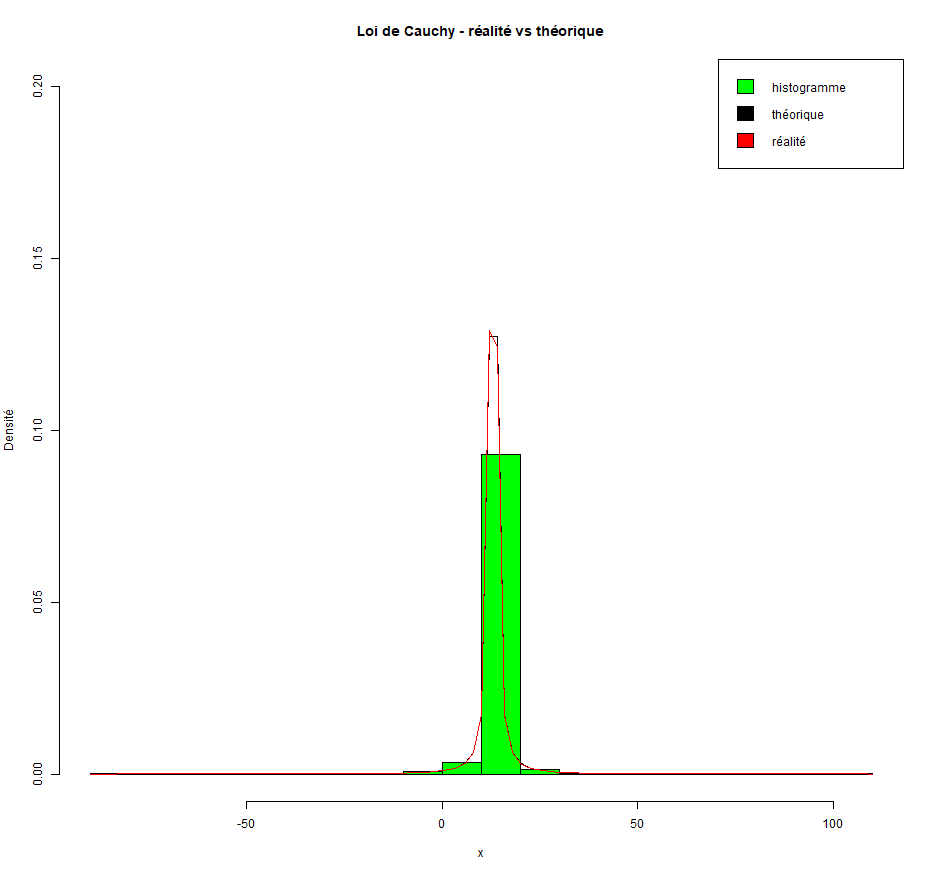
\includegraphics[width=\linewidth]{images/Cauchy_breaks=20.png}
\caption{Représentation de l'histogramme et de la courbe de densité}
\end{figure}

Les valeurs trouvées par R, $\hat{x_0} = 12.9877139$ et $\hat{a} = 0.4951073$, sont vraiment approchées à celles théoriques.

\begin{thebibliography}{3}
\bibitem{WikiLoiCauchy}

Wikipedia,

\url{https://en.wikipedia.org/wiki/Cauchy_distribution}

\end{thebibliography}
\end{document}